%
% Example Workshop Handout with title page and a section demonstrating
% the different environments defined in the top matter
%
\documentclass[a4paper,12pt,twoside]{memoir}
\usepackage{btp}    % Use the trainermanual package option (i.e. \usepackage[trainermanual]{btp}) to generate the Trainer's version of the manual
\usepackage{url}
\usepackage{underscore}
\usepackage{color}

\usepackage{graphicx}
\DeclareGraphicsExtensions{.pdf,.png,.jpg}
\graphicspath{ {./images/} }

\usepackage[T1]{fontenc}

% Set some Workshop specific info
\setWorkshopTitle{Introduction To Linux/Ubuntu \& Shell Scripting}
\setWorkshopVenue{Adelaide, South Australa}
\setWorkshopDate{October 2014}
\setWorkshopAuthor{Steve Pederson\\
Bioinformatics Centre\\
University Of Adelaide}


\begin{document}

%
% Workshop Title Page
%
\workshoptitlepage

\chapter{Introduction}

Thank you for your attendance \& welcome to the Introduction to Linux/Ubuntu \& Shell Scripting Workshop.
This is a free offering by the University of Adelaide, Bioinformatics Hub which is a centrally funded initiative from the Department of Vice-Chancellor (Research), with the aim of assisting \& enabling researchers in their work.
Training workshops \& seminars such as this one  are an important part of this initiative. 
The Bioinformatics Hub itself has a web-page at \url{http://www.adelaide.edu.au/bioinformatics-hub/}, and to be kept up to date on upcoming events and workshops, please join the internal Bioinformatics mailing list on \url{http://list.adelaide.edu.au/mailman/listinfo/bioinfo}.\\

Today's workshop has been put together based on previous material and courses prepared by Dr Stephen Bent (\textit{Robinson Institute)}, with generous technical support \& advice provided by Dr Nathan Watson-Haigh (\textit{ACPFG}) and Dr Dan Kortschak (\textit{Adelaide University, Adelson Research Group}). 
We hope it will be useful in enabling you to continue and to advance your research.\\

\section{Course Summary}
In today's workshop, the morning session will be spent introducing you to the basic tools and concepts required for data handling.
An optional afternoon session will enable you to develop these skills to a more advanced level,with progress being made more at your own pace.\\

The majority of data handling and analysis required in the field of bioinformatics uses the \textit{command line}, alternatively known as the terminal or the \textit{bash shell}.
This is a text-based interface in which commands must be typed, as opposed to the Graphical User Interfaces (aka GUIs) that most of us have become accustomed to.
Being able to access your computer using these tools enables you to more fully utilise the power \& capabilities of your machine, for both Linux \& Mac operating systems, and to a lesser extent will even enable you to dig deeper on a Windows system.\\

During the afternoon session, we will begin to write what are known as \textit{shell scripts}.
These are essentially simple programs that utilise the inbuilt functions of the shell, and can be easily used to automate processes such as de-multiplexing read libraries, or aligning reads to the genome.


\section{Icons \& Symbols}
The following set of symbols will be used throughout this document to assist you finding your way: \\

\begin{information}
Important information.\\
\end{information}

\begin{note}
Things to note.\\
\end{note}

\begin{warning}
A warning which needs to be read very carefully.\\
\end{warning}

\begin{steps}
Instructions for you to perform. \\
\end{steps}

\begin{questions}
Questions for you to answer. \\
\begin{answer}
There is no answer
\end{answer}
\end{questions}

\begin{bonus}
An optional bonus section for those progressing rapidly. \\
\end{bonus}

\begin{advanced}
An optional advanced section for those progressing very rapidly or to be used for future reference. \\
\end{advanced}

\section{Computer Setup}
\begin{information}
We will all be working on our own computers today, and will be accessing Virtual Machines running the Ubuntu operating system on the Nectar Research Cloud (\url{http://nectar.org.au/}).
The software client NoMachine (\url{https://www.nomachine.com/}), which you will have already installed, enables us to access these machines in a familiar Desktop style, even though the majority of our time will be spent within the terminal. \\

NoMachine session files will be provided to each attendee which have been pre-configured to enable easy access to these machines.
These machines are effectively dual-core machine with 8GB of RAM \& 70GB of hard drive space.
Whilst relatively small, this will be more than enough to become
familiar with the important concepts for the day.
To begin today's session, simply click (or double-click) on the
NoMachine session file that you have been given.
The desktop from the Virtual Machine (VM) that you have connected to will appear on the
NoMachine client. \\
\end{information}

\begin{figure}[h!]
  \centering
    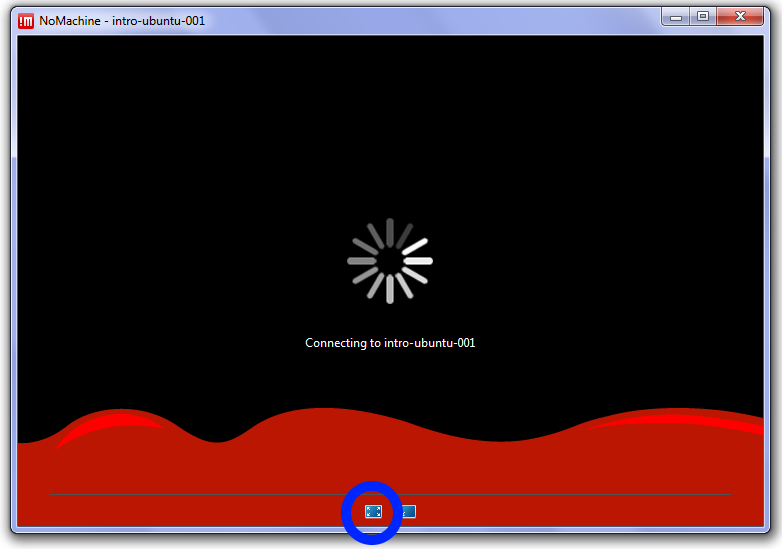
\includegraphics[width=0.8\textwidth]{NoMachine}
\end{figure}

While this is connecting, select the button circled in blue above.
This will resize NoMachine to be full screen to feel more like you are physically located at the VM.
If any security warnings appear, ignore them \& continue connecting.


\section{The Ubuntu Desktop}
\begin{note}
Now that you are connected, you will notice we are in a standard graphical environment.
The default Desktop in Ubuntu is Unity, but what we are seeing is known as the Gnome Desktop.
It's easier to load this via NoMachine, but the two variants are not dissimilar.
As many of us are used to seeing, there are click-able icons on the desktop, and drop-down menus. \\

Although we won't be using it today, Ubuntu has an built-in Office Suite of
programs which you can access from the \textit{Applications \textgreater Office} menu item.
This is where links can be found to open Document Viewer (a .pdf viewer), Libre Office Calc (Excel-like), Libre Office Writer (Word-like) \& other standard members of Office Program Suites. \\

The two main interfaces we will be using today are the \texttt{terminal} and a text editor named \texttt{gedit}.
They will appear as icons on the desktop, but can also be accessed from the drop-down menus.
\end{note}

\clearpage
\chapter{The Command Line}
\section{Initial Goals}
\begin{enumerate}
\item Gain familiarity and confidence within the Linux command-line environment
\item Learn how to navigate directories, as well as to copy, move \& delete the files within them
\item Look up the name of a command needed to perform a specified task
\end{enumerate}


\section{Background}
Command-line tools are the mainstay of analysis of large data sets.
Good candidate examples for command-line analysis are:
\begin{itemize}
\item Files that are too large to open on your computer using a text editor or Excel
\item Manipulations of data which are repetitive or laborious to perform manually
\item Any analysis that is different from what is available in programs with graphical interfaces.
\end{itemize}  

\clearpage
\section{Finding your way around}
\begin{information}
Firstly we need to open a terminal, so either click on the terminal icon on the desktop, or go to \textit{Applications \textgreater Accessories \textgreater Terminal} on the drop-down menu at the top-left of your screen.
You will notice the text \texttt{trainee@intro-ubuntu-XXX:\~{}\$} where \texttt{trainee} is the username that we have assigned to you, and \texttt{intro-ubuntu-XXX} indicates which virtual machine you have been assigned to.
The tilde is actually your current directory (see below), whilst the dollar sign just indicates the end of the address \& the beginning of where you will type commands. \\
\end{information}

\subsection{Where are we?}
\begin{steps}
Type the command \texttt{pwd} in the terminal and you will see the output \texttt{/home/trainee}.
\begin{lstlisting}
pwd
\end{lstlisting}
The command \texttt{pwd} is what we use for \underline{\textbf{p}}rinting the current (i.e. \underline{\textbf{w}}orking) \underline{\textbf{d}}irectory.
This is what will be referred to as your \textit{home directory} for the remainder of the workshop.
This is also the information that the tilde represents as a shorthand version, so whenever you see the tilde in a directory path, this is interpreted as meaning \texttt{/home/trainee}. \\
\end{steps}

\begin{warning}
\Large{Note for Mac Users Only:}\\
\normalsize{In the following code fragments, the Mac font coding system may change the tilde (\~{}) to an exclamation point (!).
This seems unavoidable \& inexplicable so if you are viewing, or have printed these notes using a Mac, wherever you see an exclamation mark in a code fragment, please interpret this as a tilde.}
\end{warning}

\begin{information}
In the above command, the home directory began with a slash, i.e. \texttt{/}.
On a Linux-based system, this is considered to be the root directory of the file system. 
Windows users would be more familiar with seeing \texttt{C:\textbackslash} as the root of the drive, and this is an important difference in the two directory structures.
Note also that whilst Windows uses the backslash (\textbackslash) to indicate a new directory, a Linux-based system uses the forward slash (/), or more commonly just referred to simply as ``slash'', marking another key difference between the two. \\
\end{information}

\begin{warning}
Although we haven't directly discovered it yet, a Linux-based file system such as Ubuntu or Mac OS-X is also \textit{case-sensitive}, whilst Windows is not.
For example, the command \texttt{PWD} is completely different to \texttt{pwd} and if \texttt{PWD} is defined in your shell, you will most likely get completely different results than from the intended \texttt{pwd} command.
\end{warning}

\subsection{Changing Directories}
\begin{information}
The command \texttt{pwd} is an example of a \textit{command} that is built into the shell.
Another built-in command is \texttt{cd} which we use to \textbf{\underline{c}}hange \textbf{\underline{d}}irectory.
No matter where we are in a file system, we can move up a directory in the hierarchy by using the command 
\begin{lstlisting}
cd ../
\end{lstlisting}
The string ``\texttt{..}'' is the convention for ``\textit{one directory above}'', whilst a single dot represents the current directory. \\
\end{information}

\begin{steps}
Enter the above command and notice that the location immediately to the left of the \$ is now given as \texttt{/home}.
This is also what will be given as the output if we enter the command \texttt{pwd}.
If we now enter \texttt{cd ../} one more time we will be in the root directory of the file system.
Try this and print the working directory again.
As detailed earlier, the output should be the root directory given as \texttt{/}. \\
\end{steps}

We can change back to the original location by entering one of either:
\begin{steps}
\begin{lstlisting}
cd /home/trainee
\end{lstlisting}
or \\
\begin{lstlisting}
cd ~ 
\end{lstlisting}
or even just \\
\begin{lstlisting}
cd
\end{lstlisting}
\end{steps}

\begin{information}
An \textit{absolute path} on Linux will always begin with the root directory symbol, e.g. \texttt{/path} would refer to a directory called \texttt{path} in the root directory of the file system.
In contrast, a \textit{relative path} can begin with either the current directory (indicated by \texttt{./}) or a higher-level directory (indicated by \texttt{../} as mentioned above).
A subdirectory \texttt{path} of the current directory could thus be specified as \texttt{./path}, whilst a subdirectory of the next higher directory would be specified by \texttt{../path}. 
Another common relative path is the one mentioned right at the start of the session, specified with \~{}, which stands for your home directory.\\
\end{information}

We can also move through multiple directories in one command by separating them with the forward slash ``\texttt{/}''.
For example, we could also get to the root directory from our home directory by typing \\
\begin{lstlisting}
cd ../../ 
\end{lstlisting}

\begin{steps}
Using the above process, return to your home directory.
\texttt{/home/trainee}. \\
\end{steps}

\subsection{Looking at the Contents of a Directory}
\begin{steps}
There is another built-in command ``\texttt{ls}'' that we can use to \textbf{\underline{l}}i\textbf{\underline{s}}t the contents of a directory.
Enter the \texttt{ls} command as it is and it will print the contents of the current directory. \\
\begin{lstlisting}
ls 
\end{lstlisting}
\end{steps}

\begin{steps}
Alternatively, we can specify which directory we wish to view the contents of, without having to change into that directory.
We simply type the \texttt{ls} command, followed by a space, then the directory we wish to view the contents of.
To look at the contents of the root directory of the file system, we simply add that directory after the command \texttt{ls}. \\
\begin{lstlisting}
ls /
\end{lstlisting}
\end{steps}

Here you can see a whole raft of directories which contain the vital information for the computer's operating system.
Among them should be the \texttt{/home} directory which is one level above your own home directory. \\

\begin{questions}
 Try to think of two ways we could inspect the contents of the \texttt{/home} directory from your own home directory. \\
\begin{answer}
\texttt{ls /home} \\
or \\
\texttt{ls ../} \\
\end{answer}
\end{questions}

\begin{note}
Notice that there are two entries in the \texttt{/home} directory. 
One is your home directory (\texttt{/home/trainee}), whilst the other is the default home directory that came with the VM (\texttt{/home/ubuntu}) before we setup your home directory.
The directory \texttt{/home} actually contains the home directories for all users, hence why there is a \texttt{/home} directory that sits one level above your own home directory.
Also note that if we ever refer to this directory, we will write it as \texttt{/home}, whereas your personal home directory is referred to without the preceding forward-slash, and will also be written in normal text font instead of the font we specifically use for code. \\
\end{note}

\begin{information}
When working in the terminal, you can scroll through your previous commands by using the up arrow to go backward, and the down arrow to move forward.
This can be a big time saver if you've typed a long command with a simple typo, or if you have to do a series of similar commands.
\end{information}

\subsection{Going Even Deeper}
\begin{information}
So far, the commands we have used were given either without the use of any subsequent arguments, e.g. \texttt{pwd} \& \texttt{ls}, or with a specific directory as the second argument, e.g. \texttt{cd ../} \& \texttt{ls /home}.
Many commands have the additional capacity to specify different options as to how they perform, and these options are often specified between the command name, and the file being operated on.
The \texttt{ls} command can be given with the option \texttt{-l} specified between the command \& the directory.
This options gives the output in what is known as \textit{long listing} format. \\
\end{information}

\begin{steps}
Inspect the contents of your home directory using the long listing format. \\
\begin{lstlisting}
ls -l ~
\end{lstlisting}
\end{steps}

The above will give three lines of output.
The first line will be something similar to
\begin{center}
\colorbox{black}{\texttt{\textcolor{white}{drwxr-xr-x 2 trainee trainee 4096 mmm dd hh:mm} \textcolor{cyan}{\textbf{Desktop}}}}\\
\end{center}

\begin{information}
The important thing to notice is that the word \textcolor{cyan}{\texttt{Desktop}} at the end of the line will be coloured \textcolor{cyan}{\textbf{blue}}, indicating that it is a directory.
The letter `\texttt{d}' at the beginning of the initial string of codes \texttt{drwxr-xr-x} also indicates this fact.
Formally, these letter are known as flags which identify key attributes about each file or directory.
We can ignore the fine detail in the rest of these flags until this afternoon (or see the bonus section), but the values \texttt{rwx} simply refer to who is able to \textbf{\underline{r}}ead, \textbf{\underline{w}}rite or e\textbf{\underline{x}}ecute the contents of the file or directory. 
These are very helpful attributes for data security \& protection against malicious software.\\

The entries \texttt{trainee trainee} respectively refer to who is the owner of the directory \& to which group it belongs.
Again, this information won't be particularly relevant to us today, so we can ignore this until later in our programming careers.
Finally, the value \texttt{4096} is the size of the directory structure in bytes, whilst the date \& time refer to when the directory was created.\\

\begin{bonus}
The flags we saw at the beginning of the entries above have a clearly defined structure. 
The first entry shows the file type and for most common files, this entry will be the ``-'' seen above.
The next entries are three triplets which refer to 1) the file's owner, 2) the current user \& 3) all users.
\end{bonus}

The last line of the output you see will be: 
\begin{center}
\colorbox{black}{\texttt{\textcolor{white}{-rwxr-{}-r-{}- 1 trainee trainee 8445 Apr 17 2012} \textcolor{green}{\textbf{examples.desktop}}}}\\
\end{center}
Notably the name of this file will be in \textcolor{green}{\textbf{green}}, indicating that it is a file not a directory.
There is also a `\texttt{-}' instead of a `\texttt{d}' at the beginning of the initial string of flags. 
The remainder of the information is essentially the same as for the directory \texttt{Desktop}.\\
\end{information}

\begin{advanced}
There are many more options that we could specify to give a slightly different output from the \texttt{ls} command.
Two particularly helpful ones are the options \texttt{-h} and
\texttt{-R}.
We could have specified the previous command as \\
\begin{lstlisting}
ls -l -h ~
\end{lstlisting}

This will change the file size to \textit{``human-readable''} format, whilst leaving the remainder of the output unchanged.
Try it \& you will notice that where we initially saw \texttt{4096} bytes, the size is now given as \texttt{4.0K}.
This can be particularly helpful for larger files, as most NGS files are very large indeed.\\

The option \texttt{-R} tells the \texttt{ls} command to look through each directory recursively.
If we enter \\
\begin{lstlisting}
ls -l -R ~
\end{lstlisting}

the output will be given in two sections.
The first is what we have seen previously, but following that will be the contents of the directory \texttt{/home/trainee/Desktop}.
It should become immediately clear that the output from setting this option can get very large \& long depending on which directory you start from.
It's probably not a good idea to enter \texttt{ls -l -R /} as this will print out the entire contents of your file system. \\

In the case of the \texttt{ls} command we can actually specify all the above options together in the command \\
\begin{lstlisting}
ls -lhR ~
\end{lstlisting}

This can often save some time, but it is worth noting that not all programmers write their commands in such a way that this convention can be followed.
The built-in shell commands are usually fine with this, but many NGS data processing functions do not accept this convention. \\
\end{advanced}

\begin{warning}
{\Huge Don't Panic!!!}\\
It's easy for things to go wrong when working in the command-line, but if you've accidentally set something running which you need to exit or if you can't see the command prompt, there are some simple options for stopping a process \& getting you back on track.
Four options to try are: \\
\begin{tabular}{p{4cm} p{8cm}}
\centering
 & \\
 \texttt{q} & quit the current process \\
 \texttt{Ctrl-c} & kill the current job \\
 \texttt{Ctrl-d} & end of input \\
 \texttt{Ctrl-z} & pause the current job, however it will need to be
 killed later. See \texttt{man kill} or \texttt{man killall} for details on how to kill a process. \\

\end{tabular}
\end{warning}

\clearpage
\section{Exploring Commands In More Detail}

\begin{information}
In order to help us find what options are able to be specified, every command built-in to the shell has a manual, or a help page which can take some time to get familiar with.
These help pages are displayed using the pager known as \texttt{less} which will display text in the terminal window, without allowing us to edit the text. \\
\end{information}

\begin{steps}
To display the help page for \texttt{ls} enter the command \\
\begin{lstlisting}
man ls
\end{lstlisting}
As beforehand, the space between the two is important \& in the first word we are invoking the command \texttt{man} which then looks for the manual associated with the command \texttt{ls}.
To navigate through the manual page, we need to know a few shortcuts which are part of the \texttt{less} pager, which allows us to view text but not edit it. \\
\end{steps}

\begin{information}
Although we can navigate through the \texttt{less} pager using up \& down arrows on our keyboards, some helpful shortcuts are:\\

\begin{center}
   \begin{tabular}{p{4cm} p{8cm}}
     \hline
     \textless\texttt{enter}\textgreater & go down one line \\
     \textless\texttt{spacebar}\textgreater & go down one page (i.e. a screenful) \\
     \textbf{b} & go up (i.e. \textbf{\underline{b}}ackwards one page) \\
     \textless & go to the beginning of the document \\
     \textgreater & go to the end of the document \\
     \textbf{q} & exit (i.e. \textbf{\underline{q}}uit the page) \\
     \hline
   \end{tabular}
\end{center}
\end{information}

\begin{questions}
Look through the manual page for the \texttt{ls} command.
If we wanted to hide the group names in the long listing format, which extra options would we need set when searching our home directory? \\

\begin{answer}
\texttt{ls -l -G ~} \\ 
or \\ 
\texttt{ls -lG ~} \\ 
or \\
\texttt{ls -o ~} \\
It may also be worth explaining to people that the \texttt{trainee} shown in the output is the file owner, not the group. \\
\end{answer}


How could we give the directory contents in long listing format, sorted by file size? \\
\begin{answer}
\texttt{ls -l -S ~} \\
or \\
\texttt{ls -lS ~} \\
\end{answer}
\end{questions}

\begin{bonus}
We can actually find out more about the \texttt{less} pager by calling it's own \texttt{man} page.
Type the command \\
\begin{lstlisting}
man less
\end{lstlisting}
 and the complete page will appear.
This can look a little overwhelming, so try pressing \texttt{h} which will take you to a summary of the shortcut keys within \texttt{less}.
There are a lot of them, so try out a few to jump through the file. \\

A good one to experiment with would be to search for patterns within the displayed text by prefacing the pattern with a forward slash.
Try searching for a common word like \textit{``the''} or \textit{``to''} to see how the function behaves, then try searching for something a bit more useful. \\
\end{bonus}

\subsection{Accessing Manuals or Help Pages}
\begin{information}
As well as entering the command \texttt{man} before the name of a command you need help with, you can often just enter the name of the command with the options \texttt{-h} or \texttt{-{}-help} specified.
Note the convention of a single hyphen which indicates an individual letter will follow, or a double-hyphen which indicates that a word will follow.
Unfortunately the methods can vary a little from command to command, so if one method doesn't get you the manual, just try one of the others. \\
\end{information}

\begin{questions}
Try accessing the manual for the command \texttt{man} all three ways. 
Was there a difference in the output depending on how we asked to view the manual?\\
\begin{answer}
Yes.
Accessing the manual using \texttt{man man} displayed it a page at a time using \texttt{less}.
The other two options just printed the entire contents all at once.\\
\end{answer}


Could we access the help page for the command \texttt{ls} all three ways? \\
\begin{answer}
No.
The option \texttt{-h} gives the output in human readable format.
However, the other two methods work.\\
\end{answer}
\end{questions}

\subsection{Some Useful Commands}
\begin{steps}
So far we have explored the commands \texttt{pwd}, \texttt{cd}, \texttt{ls} \& \texttt{man} as well as the pager \texttt{less}.
Inspect the \texttt{man} pages for the commands in the following table  \& fill in the appropriate fields.
Have a look at the useful options \& try to understand what they will do if specified when invoking the command. \\

\begin{center}
\renewcommand{\arraystretch}{1.6}
\begin{tabular}{|p{2cm} | p{8.5cm} | p{4.5cm}|}
\hline
\textbf{Command} & \textbf{Description of function} & \textbf{Useful options} \\ \hline
\texttt{man} & Display on-line manual & -k (search for keywords if you don't know the command) \\ \hline
\texttt{pwd} & Print working directory, i.e show where you are & none commonly used \\ \hline
\texttt{ls} & List contents of a directory & -a, -h, -l \\ \hline
\texttt{cd} & Change directory & (scroll down in \texttt{man builtins} to find \texttt{cd}) \\ \hline
\texttt{mv} & & -b, -f, -u \\ \hline
\texttt{cp} & & -b, -f, -u \\ \hline
\texttt{rmdir} & & \\ \hline
\texttt{mkdir} & & \\ \hline
\texttt{rm} & & -r (careful...) \\ \hline
\texttt{cat} & & \\ \hline
\texttt{less} & & \\ \hline
\texttt{wc} & & -l \\ \hline
\texttt{head} & & -n\# (e.g., -n100) \\ \hline
\texttt{tail} & & -n\# (e.g., -n100) \\ \hline
\texttt{echo} & & \\ \hline
\texttt{passwd} & & \\ \hline
\end{tabular}
\end{center}
\end{steps}

\begin{bonus}
\begin{questions}
Sometimes the side effects of a command can also be useful. 
Look at the \texttt{man} page for the command \texttt{touch} \& see if you can think of a very common usage of this command. \\
\begin{answer}
We can use \texttt{touch} to create an empty file using the command string \texttt{touch filename}.
\end{answer}
\end{questions}
\end{bonus}

\subsection{Tab auto-complete}
\begin{information}
A very helpful \& time-saving tool in the command line is the ability to automatically complete a command, file or directory name using the \texttt{\textless tab \textgreater} key.
Try typing \texttt{ls /home/tr} \& then hit the \texttt{\textless tab \textgreater} key.
Notice how the word \texttt{trainee} is completed automatically!
This functionality will automatically fill as far as it can until conflicting options are reached.
In this case, there was only one option so it was able to complete all the way to the end of the file path. \\

Now enter \texttt{head \~{}/Do} \& hit \texttt{\textless tab \textgreater}, and it will fill up to the end of the path \texttt{head \~{}/Documents/}.
Keep typing by adding \texttt{tr} immediately after the last slash symbol (i.e. no spaces) \& hit \texttt{\textless tab \textgreater} once again and it will complete up to the end of the path \texttt{head \~{}/Documents/trainingData}.
Now add the letter \texttt{p} \& hit \texttt{\textless tab \textgreater}. 
This time it will give you up to \texttt{head \~{}/Documents/trainingData/pair}, so hit \texttt{\textless tab \textgreater} again and it will show you the two options \texttt{pair1.fq} or \texttt{pair2.fq}.
The original auto-complete was unsure which one you wanted so it filled as far as it could.
The next strike of the \texttt{\textless tab \textgreater} key asked the shell to show what choices you have, so choose one of them (i.e. type 1 or 2), then hit \texttt{\textless tab \textgreater} \& the auto-complete will once again finish to the end of the file name.

This can be used to also find command names.
Type in \texttt{he} followed by two strike of the \texttt{\textless tab \textgreater} key and it will show you all of the commands that being with the string \texttt{he}, such as \texttt{head}, \texttt{help} or any others that may be installed on your computer.
If we'd hit the \texttt{\textless tab \textgreater} key after type \texttt{hea}, then the command \texttt{head} would have auto-completed, although obviously this wouldn't have saved you any typing.
\end{information}

\section{Putting It All Together}
Now we can use some the above commands to perform something useful. \\

\begin{steps}
First, let's create a personal directory under \texttt{/home/trainee} with your firstname as the directory name.
Where you see \textit{firstname} below, use your actual firstname. \\
\begin{lstlisting}
cd ~
mkdir firstname
\end{lstlisting}
\end{steps}

\begin{steps}
In the \texttt{\~{}/Documents/trainingData} directory, you will find the file \texttt{pair1.fq}
We can copy this to our newly created directory using the command \\
\begin{lstlisting}
cp ~/Documents/trainingData/pair1.fq ~/firstname/pair1.fq
\end{lstlisting}
Next we will rename the file \\
\begin{lstlisting}
mv ~/firstname/pair1.fq ~/firstname/RADSeqReads1.fq
\end{lstlisting}

We can look at the first 5 lines of the file using \\
\begin{lstlisting}
head -n5 ~/firstname/RADSeqReads1.fq
\end{lstlisting}
Or we can look at the last 10 lines of the file using \\
\begin{lstlisting}
tail -n10 ~/firstname/RADSeqReads1.fq
\end{lstlisting}
We could even page through the file using \texttt{less}
\begin{lstlisting}
less ~/firstname/RADSeqReads1.fq
\end{lstlisting}
We can even find how many lines there are in the file by using \\
\begin{lstlisting}
wc -l ~/firstname/RADSeqReads1.fq
\end{lstlisting}
\end{steps}

\begin{note}
For all the above commands we could have used the auto-complete
feature of the bash terminal.
Once you start typing the name of a file or directory, hit the
\textless \texttt{tab}\textgreater key and it will auto-complete as far as it can go.
For example, if you have two directories with one called
\texttt{\~{}/Documents} and the other called \texttt{\~{}/Downloads},
hitting \textless \texttt{tab}\textgreater ~after entering \texttt{\~{}/Doc} will auto-complete to \texttt{\~{}/Documents}. 
However, hitting \textless \texttt{tab}\textgreater ~after typing \texttt{\~{}/Do} will
do nothing as it won't be able to tell which directory you're
intending to type.\\
\end{note}

\begin{questions}
Did we need to enter the full file path in the above commands, or
could we have saved ourselves some effort? \\

\begin{answer}
Yes, we could have changed into the \texttt{\~{}/firstname} directory \&
just entered the file name. \\
\end{answer}

Counting the number of lines in a file which consists of NGS reads can be very informative.
Each read in \texttt{fastq} format consists of four lines: \\
1) A sequence identifier, \\
2) The actual sequence, \\
3) The `+' character (which can also be an optional repeat line for the identifier), \& \\
4) A quality score.
How could we find the number of sequences in a file? \\
\begin{answer}
Counting the number of lines \& dividing by 4 will give you the number of sequences in the file.
Although well beyond the scope of today, this could crudely be found using \\
\texttt{echo \$((\$(wc -l < filename.fq) / 4))}\\
although if there is a problem with the file, this will only give the number of sequences to an integer value.
\end{answer}
\end{questions}

\begin{note}
Looking through the first few lines of a file is often a good place to start if the file is not behaving as expected.
By doing this we can potentially diagnose problems with file headers, end-of-line markers or other unexpected problems. \\
\end{note}

In the next section of the workshop, we will learn how to search within a file using a style of text searching call \textit{regular expressions}.

\chapter{Regular Expressions}
\section{Introduction}
Regular expressions are a powerful \& flexible way of searching for text strings amongst a large document or file.
Most of us are familiar with searching for a word within a file, but regular expressions allow us to search for these with more flexibility, particularly in the context of genomics.
Instead of searching strictly for a word or text string, we can search using less strict matches.
For example, we could search for a sequence that is either \texttt{AGT} or \texttt{ACT} by using the patterns  \texttt{A[GC]T} or  \texttt{A(G|C)T}.
These two patterns will search for an  \texttt{A}, followed by either a  \texttt{G} or  \texttt{C}, then followed strictly by a  \texttt{T}.
Similarly a match to \texttt{ANNT} can be found by using the patterns \texttt{A[AGCT][AGCT]T} or  \texttt{A[AGCT]\{2\}T}. \\

Whilst the bash shell has a great capacity for searching a file to matches to regular expressions, this is where languages like \textit{perl} and \textit{python} offer a great degree more power.
The commands \texttt{awk} \& \texttt{sed} which we will look at later this afternoon also use regular expressions to great effect.

\section{The command \texttt{grep}}
The built-in command which searches using regular expressions in the terminal is \texttt{grep}.
This function searches a file or input on a line-by-line basis, making patterns split across lines more difficult to find.
This can be overcome by using regular expressions in a programming language like Python or Perl.  
The \texttt{man grep} page contains more detail on regular expressions under the \texttt{REGULAR EXPRESSIONS} header (scroll down a few pages).  
As can be seen in the \texttt{man} page, the command follows the form
\begin{lstlisting}
grep [OPTIONS] 'pattern' filename
\end{lstlisting}
The option \texttt{-E} is preferable as it it stand for Extended, which we can think of as ``Easier''.
As well as the series of conventional numbers and characters that we are familiar with, we can match to characters with special meaning, as we saw above where enclosing the two letters in brackets gave the option of matching either. \\

\begin{center}
\renewcommand{\arraystretch}{1.6}
\begin{tabular}{|p{4cm} | p{11.cm} |}
\hline
Special Character & Meaning \\ \hline
\textbackslash w & match any letter or digit, i.e. a word character \\
\textbackslash s & match any white space character, includes spaces,
tabs \& end-of-line marks \\
\textbackslash d & match any digit from 0 to 9 \\
. & matches any single character \\
+ & matches one or more of the preceding character (or pattern) \\
\** & matches zero or more of the preceding character (or pattern) \\
? & matches zero or one of the preceding character (or pattern) \\
\{x\} or \{x,y\} & matches x or between x and y instances of the preceding
character \\
\^{} & matches the beginning of a line (when not inside square brackets) \\
\$ & matches the end of a line \\
() & contents of the parentheses treated as a single pattern \\
{[}] & matches any one of the characters inside the brackets \\
{[}\^{}] & matches anything other than any of the characters in the brackets \\
| & either the string before or the string after the "pipe" (use
parentheses) \\
\textbackslash & don't treat the following character in the way you normally would. This is why the first three entries in this table started with a backslash, as this gives them their ``special'' properties, whereas placing a backslash before a `.' symbol will enable it to function as an actual dot/full-stop. \\
\hline
\end{tabular}
\end{center}

\section{Pattern Searching}
In this section we'll learn the basics of using the \texttt{grep}
command \& what forms the output can take.
In your \texttt{\~{}/Documents/trainingData} directory you can find
the file \texttt{words}. \\

\begin{steps}
Change into this directory \& page through the first few lines of the file to get an idea about what it contains. 
Make sure you're in the correct directory or else \texttt{grep} won't be able to find the file \texttt{words}. \\

Now let's try a few searches, and to get a feel for the basic syntax of the command, try to describe what you're searching for on your notes \textbf{BEFORE} you enter the command.
Do the results correspond with what you expected to see?

\begin{lstlisting}
grep -E 'fr..ol' words
\end{lstlisting}
\begin{lstlisting}
grep -E 'fr.[jsm]ol' words
\end{lstlisting}
\begin{lstlisting}
grep -E 'fr.[^jsm]ol' words
\end{lstlisting}
\begin{lstlisting}
grep -E 'fr..ol$' words
\end{lstlisting}
\begin{lstlisting}
grep -E 'fr.+ol$' words
\end{lstlisting}
\begin{lstlisting}
grep -E 'cat|dog' words
\end{lstlisting}
\begin{lstlisting}
grep -E '^w.+(cat|dog)' words
\end{lstlisting}
\end{steps}

\begin{steps}
In the above, we were changing the pattern to extract different results from the files.
Now we'll try a few different options to change the output, whilst leaving the pattern unchanged.
If you're unsure about some of the options, don't forget to consult the \texttt{man} page. \\
\begin{lstlisting}
grep -E 'louse' words
\end{lstlisting}
\begin{lstlisting}
grep -Ew 'louse' words
\end{lstlisting}
\begin{lstlisting}
grep -Ewn 'louse' words
\end{lstlisting}
\begin{lstlisting}
grep -EwC2 'louse' words
\end{lstlisting}
\begin{lstlisting}
grep -c 'louse' words
\end{lstlisting}
\end{steps}

\section{Pattern Matching in DNA sequences}
Now we can have a look through the RAD-Seq file that we moved \& renamed earlier.
Before we search the the file \texttt{RADSeqReads1.fq}, we should know what we this data actually is.
These are a small subset of 100bp reads from a RAD-Seq experiment \& are from the first sample in a set of paired reads.
Although we can't tell this directly from this file, the sequences were obtained from a rabbit affected by \textit{calicivirus}.
\begin{steps}
Change into the directory we created earlier using your name.
\end{steps}

\begin{steps}
If you inspect the data using the \texttt{head} command, you'll notice that the file is in sets of four lines, as we have mentioned earlier.
The first line contains a \textit{sequence identifier}, the second line is the \textit{sequence} itself, the third line is simply the `+' symbol \& the final line is a set of characters which correspond to \textit{quality scores} for each base.
\end{steps}

\begin{bonus}
Although we're not particularly interested in the quality scores,these letters correspond to numbers in the ASCII coding system, where the letter `A' has the value 65 \& so on until `z', which has the value 122.
Between the upper case \& lower case letters in this table are several other characters such as brackets \& the caret (\^{}) symbol.
If you're interested page through the file for a while \& notice how the quality scores are generally high, but do occasionally drop off at the end of the sequence.
You can google `ascii table' if you're interested in this.
\end{bonus}

\begin{questions}
As these reads are from the first sample in a set of paired reads, the final value in the sequence identifier is \texttt{_1}.
How could we search for a pattern just to extract the sequence identifiers? \\
\begin{answer}
\texttt{grep -E `\^{}@.+_1\$' RADSeqReads1.fq}
\end{answer}

How could we check for any sequences which may accidentally be included from the second sample in the pair of reads?
Hint: These identifiers would finish with \texttt{_2} \\
\begin{answer}
I'm hoping they will try to search for the incorrect string \\
\texttt{grep -E `\^{}@.+_2' RADSeqReads1.fq}.\\
The correct command should be: \\
\texttt{grep -E `\^{}@.+_2\$' RADSeqReads1.fq} \\
which should give no results. \\
\end{answer}

Did you find any reads from the other sample? \\
\begin{answer}
Hopefully not. Otherwise something's gone really weird...
\end{answer}
\end{questions}

\begin{steps}
Now we'll try searching for some sequences, so try the following search string. 
Does the output match what you expected? \\
\texttt{grep -En `TGCAGGCTCT' RADSeqReads1.fq}
\end{steps}

This should give lines 774, 3382, 3758, 7326, 7594 \& 9566 along with the sequence information and matching fragment highlighted in red.\\

\begin{questions}
For the following search string \\
\texttt{grep -En `TGCAGGCTCT.+(GA)\{2\}.+A\{3\}' RADSeqReads1.fq} \\
What do the following components of the pattern match to: \\
\texttt{`.+'} \\
\begin{answer}
This matches an unspecified length of any character, until the next key match is found. \\
\end{answer}

\texttt{(GA)\{2\}} \\
\begin{answer}
This matches to two repeats of the pattern GA. \\
\end{answer}

\texttt{A\{3\}}\\
\begin{answer}
This matches three `A's in a row. \\
\end{answer}

How could you find the sequence identifier for the above match?\\
\begin{answer}
\texttt{grep -EnC1 `TGCAGGCTCT.+(GA)\{2\}.+A\{3\}' RADSeqReads1.fq} or \\
\texttt{grep -EnB1 `TGCAGGCTCT.+(GA)\{2\}.+A\{3\}' RADSeqReads1.fq}
\end{answer}
\end{questions}

\chapter{More Command Line Tips \& Tricks}

\section{Redirection Using The Pipe Symbol}
\begin{information}
Sometimes we need to build up our series of commands \& send the results of one to another.
The ``pipe'' symbol (|) is the way we do this \& it can literally be taken as placing the output from one command into a pipe \& redirecting it somewhere new.
\end{information}
\begin{steps}
As a simple example, we could take the output from an \texttt{ls} command \& send it to the pager \texttt{less}.
\end{steps}
\begin{lstlisting}
ls -lh /usr/bin | less
\end{lstlisting}
Page through the output until you get bored, then hit \texttt{q} to quit.

\begin{questions}
Earlier we estimated the number of sequences in a file by counting the number of lines \& dividing by four.
Could you think of an easier way using pipe redirection? \\
\begin{answer}
We could extract the sequence identifiers \& redirect that to a line count.\\
\texttt{grep -E `\^{}@.+_1\$' \~{}/firstname/RADSeqReads1.fq | wc -l} \\
This should give 2500 as the result, although the use of @ as a valid
quality score can be problematic.
\end{answer}
\end{questions}

\section{Sending Output To A File}
\begin{information}
So far, the only output we have seen has been in the terminal, which is known as the \textit{standard output}, or \textit{stdout} for short.
Similar to the pipe command, we can redirect the output of a command to a file instead of to standard output, and we do this using the greater than symbol (\textgreater), which we can almost envisage as an arrow.
\end{information}

\begin{steps}
To collect a list of the sequence identifiers in our set of RADSeqReads \& write these to a file, we could use the command as above, but instead of directing the output to the terminal, we could write this to a file.
\end{steps}
\begin{lstlisting}
grep -E '^@.+_1' ~/firstname/RADSeqReads1.fq > SeqIDs.txt
less SeqIDs.txt
\end{lstlisting}

Once you've had a quick look at the file, exit the less pager and delete the file using the \texttt{rm} command.

\section{Text In the Terminal}
We can display a line of text in \textit{stdout} by using the command \texttt{echo}.
The most simple function that people learn to write in most languages is called \texttt{Hello World} and we'll do the same thing today.
\begin{steps}
\begin{lstlisting}
echo 'Hello World'
\end{lstlisting}
\end{steps}
That's pretty amazing isn't it \& you can make the terminal window say anything you want without meaning it.\\
\begin{lstlisting}
echo 'This computer will self destruct in 10 seconds!'
\end{lstlisting}

\begin{information}
There are a few subtleties about text which are worth noting.
Inspect the \texttt{man echo} page \& note the effects of the \texttt{-e} option.
This allows you to specify tabs, new lines \& other special characters by using the backslash to signify these characters.
This is an important concept \& the use of a backslash to ``escape'' normal meaning of a character is very common.
Try the following three commands \& see what effects these special characters have.
\end{information}
\begin{steps}
\begin{lstlisting}
echo 'Hello\tWorld'
echo -e 'Hello\tWorld'
echo -e 'Hello\nWorld'
\end{lstlisting}
\end{steps}

\begin{steps}
We can also evaluate numerical expressions in the terminal window using the echo command, with the numerical expression prefaced by the dollar sign \& the expression enclosed in double brackets. \\
\begin{lstlisting}
echo $((1+2))
echo $((10^2))
\end{lstlisting}
As you may have noticed, that last command didn't work as you might have expected, so always be vary careful performing these types of calculations.
The standard arithmetic processes like addition, subtraction, division \& multiplication will work as expected, but most programmers don't really use this functionality terribly much.
\end{steps}

\section{sed: The Stream Editor}
\begin{information}
One very useful command in the terminal is \texttt{sed}, which is short for \textit{stream editor}.
Instead of the \texttt{man} page for \texttt{sed} the \texttt{info sed} page is larger but a little easier to digest.
This is a very powerful command which can be a little overwhelming at first.
If using this for your own scripts \& you can't figure something out, remember ``Google is your friend'' \& sites like \url{www.stackoverflow.com} are full of people wrestling with similar problems to you.
These are great places to start looking for help \& even advanced programmers use these tools. \\
\end{information}

For today, there are two key \texttt{sed} functionalities that we want to introduce.\\
\begin{enumerate}
\item Using \texttt{sed} to alter the contents of a file/input;
\item Using \texttt{sed} to print regions of a file
\end{enumerate}

\subsection*{Altering a file or other input}
\texttt{sed} uses \textit{regular expressions} that we have come across under the \texttt{grep} section, and we can use these to replace strings or characters within a text string.
The command works in the form \texttt{sed `SCRIPT' INPUT}, and the script section is where all the action happens.
Input can be given to \texttt{sed} as either a file, or just as a text stream via the \textit{pipe} that we have already introduced.

\begin{steps}
In the following example the script begins with an `s' to indicate that we are going to make a substitution.
The beginning of the first pattern (i.e. the \textit{regexp} we are searching for) is denoted with the backslash, with the identical delimiter indicating the replacement pattern, and this is in turn completed with the same delimiter.
Try this simple example from the link \url{http://www.grymoire.com/Unix/Sed.html} which is a very detailed \& helpful resource about the usage \texttt{sed}.
Here we are sending the input to the command via the pipe, so no `INPUT' section is required: \\
\begin{lstlisting}
echo Sunday | sed 's/day/night/' 
\end{lstlisting}
Here you are passing \texttt{sed} the string Sunday, and \texttt{sed} takes day and turns it into night.  
\texttt{sed} will only replace the first instance of the string on any line, so try: \\
\begin{lstlisting}
echo Sundayday | sed 's/day/night/' 
\end{lstlisting}
It only replaced the first instance of day and left the second.  You can make it 'global', where it switches every instance by using the `g' option at the end of the pattern like this: \\
\begin{lstlisting}
echo Sundayday | sed 's/day/night/g' 
\end{lstlisting}
You can `capture' parts of the pattern in parentheses and access that in the second part of the regular expression (what you are switching to) using \textbackslash 1, \textbackslash 2, etc., to denoted the number of the captured string.
If you want to match `ATGNNNTGA', where N is any base, and replace those three bases with an expanded repeat of them', you could do the following where we capture the undefined string between \texttt{ATG} \& \texttt{GTA}, and expand it: \\
\begin{lstlisting}
echo 'ATGCCAGTA' | sed -r 's/ATG(.{3})GTA/ATG\1\1\1GTA/g'
\end{lstlisting}
The \textbackslash 1 take the contents of the first parenthesis and uses it in the substitution, even though you don't know what the bases are.
Note that the `-r' option was set for this, which turns on extended regular expression capabilities.
This can be a powerful tool \& multiple parentheses can be used: \\
\begin{lstlisting}
echo 'ATGCCAGTA' | sed -r 's/(ATG)(.{3})(GTA)/\3\2\2\1/g'
\end{lstlisting}
In this command we switched the order of the first \& last triplet, and expanded the middle unknown string twice.
Note how quickly this starts to look confusing though!
Taking care to be clear when writing these types of procedures can be an important idea when you have to go back \& re-read your code a year or two later.
(Yes this will happen a lot!!!)
\end{steps}

\begin{information}
The use of backslashes to delineate each section of the script used by \texttt{sed} is the most common convention, but we are not restricted to it.
We could have uses any `wild-card' type character to follow the `s', such as `*' `:' or `\%' although this must be consistent across all sections of the script, and should only be used if the backslash itself is part of the search or replacement string.
\end{information}

\subsection*{Displaying a region from a file}
The command \texttt{sed} can also be used to replicate the functionality of the \texttt{head} \& grep commands, but with a little more power at your fingertips.
By default \texttt{sed} will print the entire input stream it receives, but setting the option `-n' will turn this off.
Try this by adding an `n' immediately after the `-r' in one of the above lines \& you will notice you receive no output.
This is useful if we wish to restrict our output to a subset of lines within a file, and by including a `p' at the end of the script section, only the section matching the results of the script will be printed.
\begin{steps}
Make sure you are in the \texttt{\~{}/firstname} directory \& we can look through the file \textit{RADSeqReads1.fq} again.
\begin{lstlisting}
sed -n '1,10 p' RADSeqReads1.fq
\end{lstlisting}
This will print the first 10 lines, like the \texttt{head} command will by default.
However, we could now print any range of lines we choose.
Try this by changing the script to something interesting like `101,112 p'.
We could also restrict the range to specific lines by using the \texttt{sed} increment operator `\~{}'.
\begin{lstlisting}
sed -n '1~4p' RADSeqReads1.fq
\end{lstlisting}
This will print every 4th line, beginning at the first, effectively giving just the sequence identifiers.
We could use this just to extract the sequences themselves, or the quality scores.
\end{steps}

\begin{questions}
The previous command prints every 4th line, but isn't restricted to any range within the file.
How could we restrict the output to just the first 10 identifiers? \\
\begin{answer}
We could pipe the output to another \texttt{sed} command or  to head.\\
\texttt{sed -n `1\~{}4p' RADSeqReads1.fq | sed -n `1,10 p'} \\
\texttt{sed -n `1\~{}4p' RADSeqReads1.fq | head -n10} \\
\end{answer}
\end{questions}

\begin{steps}
We can also make sed operate like \texttt{grep} by making it only print the lines which match a pattern.
\begin{lstlisting}
sed -rn '/TGCAGGCTCT.+(GA){2}.+/ p' RADSeqReads1.fq
\end{lstlisting}
Note however, that the line numbers are not present in this output.
\end{steps}


\section{Downloading Data}

\begin{steps}
The terminal makes obtaining data from any publicly available sources very easy using the command \texttt{wget}, once you know the location of a file.
Let's find a genome to download by opening Firefox \& heading to \texttt{ftp://ftp.ncbi.nlm.nih.gov/genomes/Bacteria/}.
Here we can see a list of all the Bacteria which have genome information available.
Open one of the folders to have a look at the contents, or if you'd like scroll down to everyone's favourite probiotic \texttt{Lactobacillus_acidophilus_30SC_uid63605}.
We'll download the \textit{General Feature Format} file with the suffix \texttt{.gff} file which contains information about any identified genomic features.
If you've chosen Lactobacillus, we'll download the file NC_015214.gff.
Right-click on the file \& select \textit{Copy Link Location}.
If you're not already in your personal directory, i.e. \texttt{\~{}/firstname} then change into this directory and type the command \texttt{wget}.
Once you've typed this command, right-click and paste the contents of the clipboard to give the following (apologies for the small font):
\end{steps}

\begin{lstlisting}[basicstyle=\tiny]
wget ftp://ftp.ncbi.nlm.nih.gov/genomes/Bacteria/Lactobacillus_acidophilus_30SC_uid63605/NC_015214.gff
\end{lstlisting}

This will download the selected file into your current working directory.
Don't forget to have a look at the \texttt{man} page to make sure you understand how the command works.

\begin{steps}
The first 5 lines of this file is what we refer to as a \textit{header}, which contains important information about how the file was generated in a standardised format.
Many file formats have these structures at the beginning but for our purposes today we don't need to use any of this information so we can move on.
Have a look at the beginning of the file to see what it looks like.
\end{steps}
\begin{lstlisting}
head NC_015214.gff
\end{lstlisting}

Notice the header lines begin with one or two hash symbols, and the remainder of the file contains information about the genomic features.
The first feature is annotated as a \textit{region} in the third field, whilst the second feature is annotated as a \textit{gene}.

\begin{questions}
How many features are contained in this file?\\
\begin{answer}
\texttt{wc -l NC_015214.gff} \\
This will give 4355, but the first 5 lines are header lines.
To count the non-header lines you could try several things:\\
\texttt{grep -vc `\^{}\#' NC_015214.gff} \\
or\\
\texttt{grep -c `\^{}[\^{}\#]' NC_015214.gff} \\
\end{answer}
\end{questions}

\begin{advanced}
As mentioned above, this file contains multiple features such as \textit{regions}, \textit{genes}, \textit{CDSs}, \textit{exons} or \textit{tRNAs}.
If we wanted to find how many regions are annotated in this file we could use the processes we've learned above: \\
\texttt{grep -c `region' NC_015214.gff} \\

If we wanted to count how many genes are annotated, the first idea we might have would be to do something similar using a search for the pattern \texttt{'gene'}.
Try it \& you will notice immediately that adding the two numbers will give you a greater number than the number of features. \\
\begin{questions}
What is causing this problem \& how could we get around it? \\
\begin{answer}
Note that some of the occurrences of the word \textit{gene} appears in many lines which are not genes.
We need to restrict the search to one of the tab-separated fields by including a white-space character in the search.
The command:\\
\texttt{grep -En `\textbackslash sgene\textbackslash s' NC_015214.gff | wc -l} \\
will give a much different result as now we are searching for the word gene surrounded by white-space.
This is good time to mention that just because we are looking for something in one field, doesn't mean it won't appear in another field \& mess up our results.
Alternatively, we could have cut the third field \& counted the entries of the word gene: \\
\texttt{cut -f3 NC_015214.gff | grep -c `gene'}
\end{answer}
\end{questions}
\end{advanced}

\begin{information}
The file we have downloaded was an uncompressed text file. 
Often, files you download this way will be compressed (tar: tape archive) and archived (zipped). 
If you see file name suffixes like .tar, .zip, .gz, and/or .bz2, among others, that is what these are.  
You can use the commands tar, gzip, and bzip2 (look at the man pages or -{}-help option), e.g. tar -xvzf archive.tar.gz
\end{information}

\chapter{Writing Shell Scripts}
Sometimes we need to perform repetitive tasks on multiple files, or need to perform complex series of tasks and writing the set of instructions as a script is a very powerful way of performing these tasks.
They are also an excellent way of ensuring the commands you have used in your research are retained for future reference.
Keeping copies of all electronic processes to ensure reproducibility is a very important component of any research. 
Writing scripts requires an understanding of several key concepts which form the foundation of much computer programming, so let's walk our way through a few of them. \\

\section{Some Important Concepts}

Two of the most widely used techniques in programming are that of the \texttt{for} loop, and logical tests using an \texttt{if} statement.

\subsubsection*{For Loops}

A \texttt{for} loop is what we use to cycle through an input one item at a time 
\begin{steps}
\begin{lstlisting}
for i in 1 2 3; do (echo -e $i^2 = $(($i*$i))); done
\end{lstlisting}
\end{steps}

\begin{information}
In the above code the fragment before the semi-colon asked the program to cycle through the values 1, 2 \& 3, letting the variable `i' take each value in order of appearance.
First i = 1, then i = 2 \& finally i = 3.
After that was the instruction on what to do for each value.
Note that the value of the variable `i' was \textit{prefaced by the dollar sign (\$).
This is how the bash shell knows it is a variable, not the letter `i'.}
The command \texttt{done} then finished the \texttt{do} command.
All commands like \texttt{do}, \texttt{if} or \texttt{case} have completing statements, which respectively are \texttt{done}, \texttt{fi} \& \texttt{esac}.
\end{information}

\subsubsection{If Statements}
If statements are those which only have a binary `yes' or `no' response.
For example, we could specify things like:
\begin{itemize}
\item \texttt{if} (i>1) then \texttt{do} something, or
\item \texttt{if} (fileName==bob.txt) then \texttt{do} something else
\end{itemize}

\begin{information}
Notice that in the second if statement, there was a double equals sign.
This is the programmers way of saying \textit{compare} the first argument with the second argument.
A single equals sign is generally interpreted by a program as \textit{assign} the value of the first argument to be the second argument.
This use of `double operators' is very common, notably you will see \&\& to represent the command `\textit{and}', and || to represent `\textit{or}.'
A final useful trick to be aware of is the use of an exclamation mark to reverse a command.
A good example of this is the use of the command `!=' as the representation of \textit{not equal to} in a logical test.
\end{information}

\section{awk: A command and a language}
Another powerful command is \texttt{awk} which can be used as a command, as well as functioning as it's own language.
We'll just use it as a command today, and it is extremely useful for dealing with tab- or comma-separated files, such as we often see in biological data.
\begin{information}
The basic structure of an \texttt{awk} command is: 
\begin{center}
\texttt{awk `/<pattern>/' file} 
\end{center}
\texttt{awk} will then search the file and output any line containing the regular expression pattern (kind of like \texttt{grep)}.
With \texttt{awk}, you can also do: 
\begin{center}
\texttt{awk `\{<code>\}' file} 
\end{center}
where you can put a little awk program in the curly braces. 
You can specify values from different columns of the file as \$1, \$2, etc., (or you can use \$0 for the whole line).
\end{information}

\begin{steps}
We have that *.gff file and we've already looked at it at little, so let's pull out particular features!
Change into the appropriate directory \& enter
\begin{lstlisting}
awk '{if ( ($3=="gene") && ($4 > 10000) && ($4 < 20000) ) print $0}' NC_015214.gff
\end{lstlisting}
\end{steps}
\begin{note}
In the above code, \texttt{\$3==''gene''} asks for the entry in the third field to be ``gene.''
The next two fragments request for the values in the fourth field (i.e. \$4) to be between 10000 \& 20000.
Thus we have found all the features annotate as genes in a 10000bp region of this genome.
Notice that each these three commands were enclosed in a pair of brackets within an outer pair of brackets.
This gave a command of the form: \\
\texttt{( (Condition1) \&\& (Condition2) \&\& (Condition3) )} \\
After this came the fragment \texttt{print \$0} which asked \texttt{awk} to print the entire line if the 3 conditions are true.
You've just written (\& hopefully understood) a computer program!
\end{note}

\begin{steps}
Another example (what does this do?): \\
\begin{lstlisting}
awk '{if (($5 - $4 > 1000) && ($3 == "gene")) print $0}' NC_001318.gff 
\end{lstlisting}
If you don't want to output all of the columns, you can specify which ones to output.  
While we're at it, let's save the output as a file: \\
\begin{lstlisting}
awk '{if (($5 - $4 > 1000) && ($3 == "gene")) print $1, $2, $4, $5, $9}' NC_015214.gff > awkout.txt
\end{lstlisting}
\end{steps}

\section{Shell Scripts}
Now that we've been through just some of the concepts \& tools we can use when writing scripts, it's time to tackle one of our own where we can bring it all together.

\begin{information}
Every bash shell script begins with what is known as a \textit{shebang}, which we would commonly recognise as a hash sign followed by an exclamation mark, i.e \texttt{\#!}.
This is immediately followed by \texttt{/bin/bash}, which tells the interpreter to run the command \texttt{bash } in the directory \texttt{/bin}.
This opening sequence is vital \& tells the computer how to respond to all of the following commands.
As a string this looks like:\\
\begin{lstlisting}
#!/bin/bash
\end{lstlisting}
\end{information}

\begin{note}
The hash symbol generally functions as a comment character in scripts.
Sometimes we can include lines in a script to remind ourselves what we're trying to do, and we can preface these with the hash to ensure the interpreter doesn't try to run them.
It's presence as a comment here, followed by the exclamation mark, is specifically looked for by the interpreter, but beyond this comment lines are generally ignored by scripts \& programs.
\end{note}

\subsection{An Example Script}
The following is a script which will extract only the CDS features from the .gff file we have been working with, and export them to a separate file.
Look through each line carefully \& make write down your understanding of what each line is asking the program to do.

\begin{warning}
Don't try to enter these commands directly in the terminal!!!
They are designed to be placed in a script, which we will do in a minute.
\end{warning}

\begin{lstlisting}
#!/bin/bash

# Declare some helpful variables
FILEDIR=~/nectar-workshop-template/examples/intro_ubuntu_2014/files
FILENAME=NC_015214.gff
OUTFILE=NC_015214_CDS.txt

# Make sure the directory exists
if [ -d ${FILEDIR} ];
  then
    echo Changing to ${FILEDIR}
    cd ${FILEDIR}
  else
    echo Cannot find directory ${FILEDIR}
    exit 1
fi

# If the file exists, extract the important CDS data
if [ -a ${FILENAME} ];
  then
    echo Extracting CDS data from ${FILEDIR}/${FILENAME}
    echo "SeqID Source Start Stop Strand Tags" > ${OUTFILE}
    awk '{if (($3=="CDS")) print $1, $2, $4, $5, $7, $9}' ${FILENAME} >> ${OUTFILE}
  else
    echo Cannot find ${FILENAME}
    exit 1
fi
\end{lstlisting}

\begin{information}
Note that in the above script every time the value of a variable was used, it was prefaced by the \$ symbol, and the name was enclosed in curly brackets.
The \$ symbol is required, but the brackets are just a personal habit to make identification of variables easier as you skim through the code.
Similarly, the variables were defined as all capital letters for ease of identification.
It may be worth noting that most commands are strictly lower case.
\end{information}

\begin{information}
The directory \& file checking stages were also of the form if [...].
This is a curious command that checks for the presence of something. 
The options -d \& -a specify a directory or file respectively.
\end{information}

\begin{questions}
Will the above script generate a tab, comma or space delimited text file? \\
\begin{answer}
It will be space delimited. 
We could have specified tab delimited by inserting ``\textbackslash t'' between each field.
\end{answer}
\end{questions}

\begin{steps}
Open the \texttt{gedit} text editor \& save the blank file in your directory as \textit{extract_CDS.sh}.
Now write this above script into the editor, but \textit{taking care to use the directory where you have the .gff file stored in the appropriate place.}
Once you have written the script, save it \& close it.\\
\end{steps}

\subsection{Changing File Permissions}
\begin{steps}
In the directory you have saved the script, enter the \texttt{ls -l} command.
You should see the series of triplets we discussed this morning as \texttt{-rw-r-{}-r-{}-}, indicating that it is writeable by you only, but is readable by all users.
Enter the command: \\
\begin{lstlisting}
chmod +x extract_CDS.sh
\end{lstlisting}
Now repeat the \texttt{ls -l} command and you will see that the third entry in every triplet is now \texttt{x} instead of \texttt{-}.
This means that all users can now execute the file.
It is now a live computer program just waiting to be run.
Run it using the command: \\
\begin{lstlisting}
./extract_CDS.sh
\end{lstlisting}
\end{steps}

\begin{note}
Don't forget to look at \texttt{man chmod} to figure out what you did earlier.
This is a little too complex to spend time with now, but will be important to learn sooner rather than later.
\end{note}

\section{Some Challenges}
Now that we have written our first script, the challenge for the rest of the session will to be create your own script from scratch.
You can use the gedit text editor for this \& it will automatically colour code as you go, which can be very helpful for seeing where you are as you write code.

\begin{steps}
The restriction site for the RAD-Seq dataset we have is TGCAG.
In the \texttt{~/trainingData} folder, we have both pairs of reads.
Your challenge is to write a script to find:
\begin{enumerate}
\item How many reads there are in each .fq file
\item How many reads begin with the restriction site
\item Output this into a new file, with appropriate column headings. \\
\end{enumerate}
\end{steps}

\begin{steps}
The .fq files we have were processed by a program that has done strange things to the identifiers.
Each piece of information is separated by underscores, which should be colons, as specified by the defined fastq format \url{https://en.wikipedia.org/wiki/FASTQ_format#Illumina_sequence_identifiers}.
The digit indicating which member of a pair the sequence belongs to should also be of a different format, as seen in the given definition.\\

Can you write a script to change these identifiers back to the correct format? 
You can omit the machine identifier, or just make a name up if you feel like it.
\end{steps}

\end{document}
